While nano data centers are motivated by the energy consumption problem~\cite{DBLP:conf/conext/ValanciusLMDR09},
current research reveals that the advantage of the nano data centers in energy efficiency relies on certain technical foundations.
In the following chapters, this energy consumption problem and its technical challenges are discussed. Similar to the political and legal challenges, further issues will arise during the development process of nano data centers in the field of technical challenges, which are complicated to predict. The following aspects, however, need to be closely looked at. 


\subsubsection{Energy Consumption Model for Nano Data Centers} \label{sec:model}


To give an overview of the technical challenges towards nano data center development,
we first need to figure out the energy consumers of the nano data center applications.

Considering the nano data center (NaDa) platform proposed in~\cite{DBLP:conf/conext/ValanciusLMDR09},
users will host tiny managed nano servers on their end-user devices such as Triple-Play gateways and DSL/cable modems,
and communicate with each other following a Peer-to-Peer (P2P) philosophy.
Thus, suppose a user (client) wants to access the content stored in a nano server hosted by another user (manager),
the energy consumption for this process consists of~\cite{DBLP:journals/sigmetrics/JalaliAVHAT14}:
\begin{itemize}
\item the energy consumed by the client for requesting the content, denoted as $E_\text{req}$;
\item the energy consumption of the content transportation process, denoted as $E_\text{trans}$; and
\item the energy consumed by the manager for storing the content and processing the request, denoted as $E_\text{serv}$.
\end{itemize}
If we denote the total energy consumption as $E_\text{total}$, we can derive the following formula:
\begin{equation}
E_\text{total}=E_\text{req}+E_\text{trans}+E_\text{serv} \label{abstract_model}.
\end{equation}

To detail the formula from technical aspects, we need to understand the internet protocol (IP) network.
\cite{iptv} modeled the IP network as the combination of three domains:
the access network, the metropolitan and edge networks and the core network.
For centralized data center applications,
\cite{iptv} visualized the IP network model as shown in Figure~\ref{fig:ipnet}.
The access network connects each end-user to the metropolitan and edge network,
which serves as the interfaces to the core network.
Centralized data centers are usually directly connected with the core network,
but for nano data centers, since nano servers are hosted in end-user devices,
the data has to traverse the access network twice~\cite{tradeoff}.
 
\begin{figure}[h]
	\fontsize{12}{12} \selectfont
	\centerline{\resizebox{15cm}{!}{\input{image/IPnetwork.eps_tex}}}
	\caption{IPTV network model for centralized data centers~\cite{iptv}}
	\label{fig:ipnet}
	\normalsize
\end{figure}

We can now detail formula (\ref{abstract_model}) and adapt it to the energy consumption model proposed in~\cite{DBLP:journals/sigmetrics/JalaliAVHAT14} as the following:
\begin{align}
E_\text{req}&=E_{c}+E_\text{access},\\
E_\text{trans}&=E_\text{edge}\cdot h_\text{edge}+E_\text{core}\cdot h_\text{core},\\ \label{eq:trans}
E_\text{serv}&=E_\text{access}+ E_{m},
\end{align} 
where $E_c$ represents the energy consumed in the end-user device of the client, 
$E_\text{access}, E_\text{edge}$, and $E_\text{core}$ represent the energy consumed in the access network, edge network and core network, respectively, 
$h_\text{edge}$ and $h_\text{core}$ represent the number of hops in the edge and core networks,
and $E_m$ represents the energy consumed in the end-user device of the manager.

In the following, we will introduce three technical challenges that we regard as fundamental and argument our selections with respect to the proposed energy consumption model.
These challenges are:
the activation of nano servers;
the selection of the access network that the nano servers are attached to; 
and the trade-off between the distance among nano servers and the number of data replications.

\subsubsection{Activation of Nano Servers}

A nano data center platform is constructed with end-user devices as nano servers.
We refer a nano server as \textit{active}, when it is on and the user is accessing the nano data center service,
and we refer a nano server as \textit{idle}, when it is on but the user is not accessing the nano data center service.
Whenever a nano server is on,
no matters it is active or idle,
it consumes energy.
\cite{DBLP:conf/conext/ValanciusLMDR09} proposed a thorough study on how the activation status of nano servers affects the total energy consumption.
\cite{DBLP:conf/conext/ValanciusLMDR09} denoted the active time of a nano server as $t_\text{act}$ and the idle time of the nano server as $t_\text{idle}$,
and introduced a coefficient $R$ that represents the ratio of the active time of nano servers to the whole duration when nano servers are on:
\begin{equation}
R=\frac{t_\text{act}}{t_\text{act}+t_\text{idle}}.\\
\end{equation}
As proposed in~\cite{DBLP:conf/conext/ValanciusLMDR09}, 
$R$ is involved in the calculation of both $E_c$ and $E_m$ in the energy consumption model.
As a result,
the energy consumption of nano data centers correlates with $R$ as shown in Figure~\ref{fig:active},
where five different active time ratios (0.01, 0.05, 0.2, 0.5, 1) are chosen for comparison,	
and the energy consumption of a centralized data center is also shown as a reference.
We can see that the energy consumption of nano servers increases as the active time ratio decreases,
and when the ratio is large than 0.2, the energy consumption of nano servers surpasses the energy consumption of the centralized data center,
i.e. the nano data center becomes less energy efficient.

\begin{figure}[h]
	\fontsize{12}{12} \selectfont
	\centerline{\resizebox{5cm}{!}{\input{image/chart2.eps_tex}}}
	\caption{Energy consumption of nano servers with different active time ratio, and of a centralized data center~\cite{DBLP:conf/conext/ValanciusLMDR09}}.
	\label{fig:active}
	\normalsize
\end{figure}

A disappointing fact is that we cannot simply assume the active time ratio $R$ to be higher than $0.2$ most of the time.
Taking the widely-used video delivered by Internet protocol (IPTV)  as an example:
according to~\cite{DBLP:conf/conext/ValanciusLMDR09} and~\cite{watchingTV},
the IPTV user activity shows large variation throughout the day,
as shown in Figure~\ref{fig:iptv}.
Even the in the peak hour,
fewer than $20\%$ of customers are active (i.e. $R<0.2$);
as for in the midnight,
less than $5\%$ of customers are active (i.e. $R<0.05$).
On average,
the active ratio $R$ is around $0.07$,
which means that if all nano servers are on in the whole day,
it is energy \textbf{in}efficient to apply nano data centers.

\begin{figure}[h]
	\fontsize{12}{12} \selectfont
	\centerline{\resizebox{5cm}{!}{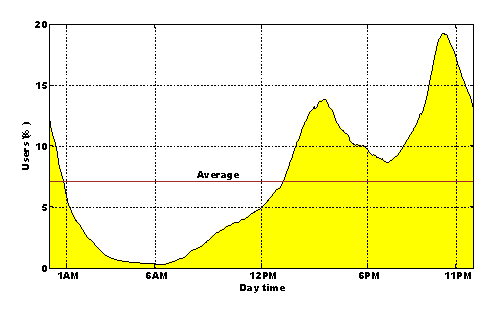
\includegraphics{image/chart3.eps}}}
	\caption{User activity of the IPTV service~\cite{DBLP:conf/conext/ValanciusLMDR09}}.
	\label{fig:iptv}
	\normalsize
\end{figure}

Therefore, to make a nano data center platform energy-efficient,
it is necessary to increase the active time ratio.
From our view,
a possible solution is to turn off the nano server time to time to reduce the idle time of the nano servers.
But for the nano servers attached to DSL-modems or other functional devices,
such as the NaDa model proposed in~\cite{DBLP:conf/conext/ValanciusLMDR09},
turning off nano servers can lead to side-effects on the usage of other internet services of users,
and thus the implementation of this solution requires further study.
Another possible solution is to modify the applications for the nano data center,
such as running multiple applications that have different peak hours,
aiming to maximize the active time of the nano servers.
So far we are unaware of any research tackling these problems,
and thus we list the activation of nano servers as one of the four technical challenges towards nano data center development.

\subsubsection{Access Network}

As discussed in Section~\ref{sec:model}, the access network connects nano servers to the edge network.
According to the analysis proposed in~\cite{tradeoff} and~\cite{DBLP:journals/sigmetrics/JalaliAVHAT14},
the power consumption of the access network needs to be counted twice for nano data centers,
i.e. $E_\text{access}$ needs to be counted both in $E_\text{req}$ and $E_\text{serv}$.
Thus, the energy efficiency of the access network has a large impact on the energy efficiency of the nano data center platform.

The energy consumption of the access network has been studied in~\cite{DBLP:journals/sigmetrics/JalaliAVHAT14} and~\cite{accessNetwork}.
Both studies refer Passive Optical Networks (PON) as energy-efficient access networks,
and indicate that wireless networks (WiMAX~\cite{accessNetwork}, 4G, WiFi~\cite{DBLP:journals/sigmetrics/JalaliAVHAT14} are relatively energy-inefficient.
Figure~\ref{fig:accessNet} shows a comparison of energy consumption between nano data centers using different access networks and centralized data centers with different energy consumption values,
where the curves for GPON and Ethernet almost overlap, and the curves for WiFi and centralized data center with 20$\mu J/$bit almost overlap.
We can see that different access networks result in huge difference of energy consumption,
and nano data centers attached to energy-inefficient access networks consume even more energy than centralized data centers.
 
\begin{figure}[h]
	\fontsize{12}{12} \selectfont
	\centerline{\resizebox{5cm}{!}{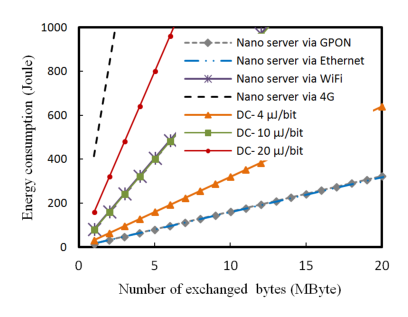
\includegraphics{image/chart.eps}}}
	\caption{A comparison of energy consumption between nano data centers using different access networks and centralized data centers with different energy consumption values~\cite{DBLP:conf/conext/ValanciusLMDR09}}.
	\label{fig:accessNet}
	\normalsize
\end{figure}

For nano data centers,
since each nano servers is possessed by an end-user,
it requires further study on the access network that these end-users may or may not use,
before one can determine whether the implementation of nano data centers can save energy or not.

Another concern regarding the access network of nano data centers is the trade-off between energy consumption and the access rate.  
Figure~\ref{fig:accessNet2} shows their correlation from two aspects.
As shown in the left figure,
for a single user,
the power consumption increases with the average access rate,
and as shown in the right figure, 
the energy per bit decreases with the average access rate.
For the two relatively energy-efficient access networks -- Point-to-Point optical access network (PtP) and PON,
their performance show different trends with the increase of the access rate.
While PON is more energy efficient for a low access rate,
it consumes more energy than PtP when the access rate surpasses 300Mb/s.
Thus, it also requires further study on the selection of the access networks with respect to the expected access rate.

\begin{figure}[h]
	\fontsize{12}{12} \selectfont
	\centerline{\resizebox{14cm}{!}{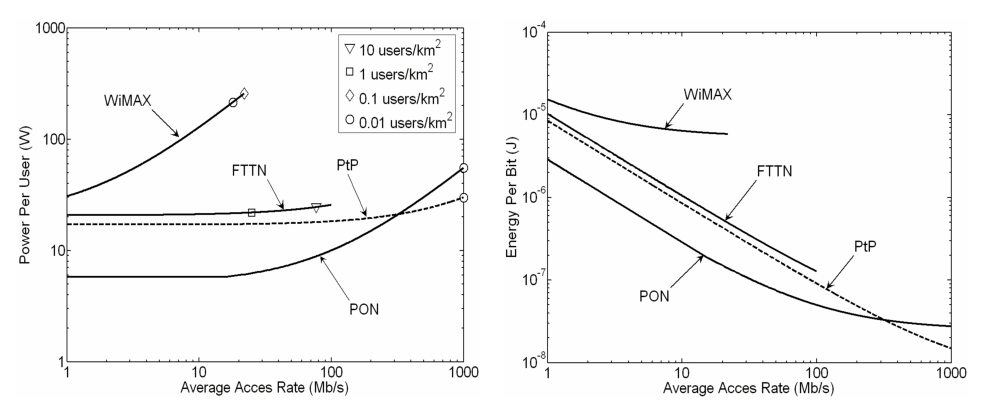
\includegraphics{image/chart4.eps}}}
	\caption{Power consumption per user for different access networks and energy per bit of different access networks~\cite{accessNetwork}}.
	\label{fig:accessNet2}
	\normalsize
\end{figure}

\subsubsection{Trade-off: Distance and Replication}

The energy consumption of the data transmission process ($E_\text{trans}$) in nano data center platforms is dependent on the number of hops in the edge ($h_\text{edge}$) and core networks ($h_\text{core}$),
as mentioned in (\ref{eq:trans}) in Section~\ref{sec:model}.
\cite{DBLP:journals/sigmetrics/JalaliAVHAT14} estimated the average number of hops in the edge and core networks to be $3$ and $5$,
using \textit{traceroute} from end-user devices to WordPress~\cite{wordpress} servers.
The number of these hops can be understood as the distance between the end-user requesting data and the end-user hosting the corresponding data.
Regarding the location of the communicating end-users,
the number of hops shows large variation:
for non-local users,
\cite{DBLP:journals/sigmetrics/JalaliAVHAT14} measured $h_\text{edge}$ and $h_ \text{core}$ as $3$ and $8$;
and for local users,
$h_\text{edge}$ and $h_\text{core}$ are measured as $1$ and $2$.
Figure~\ref{fig:location} shows the energy consumption of the the core and edge networks for the data transmission between local and non-local users,
and compares them with the centralized data center.
We can see that if an end-user accesses data from a non-local nano server, 
the energy consumption of the edge and core networks can be even higher than accessing data from a centralized data center.

\begin{figure}[h]
	\fontsize{12}{12} \selectfont
	\centerline{\resizebox{5cm}{!}{\input{image/chart5.eps_tex}}}
	\caption{Energy consumption of core and edge networks for accesing data from different locations~\cite{DBLP:journals/sigmetrics/JalaliAVHAT14}}
	\label{fig:location}
	\normalsize
\end{figure}

A natural solution to reduce or balance the data transmission distance is to add data replicas~\cite{tradeoff}~\cite{iptv}.
However,
while data replication can be beneficial to the energy-efficiency in the transmission process,
it also leads to the increase of the energy consumption for storing the data.
\cite{iptv} indicated that the data replication strategy should depend on the popularity of the data.
Figure~\ref{fig:popularity} shows the contribution of storage, servers and transmission to the total power consumption of IPTV services,
where 20 replicas of a 2-hour SD movie are stored in 20 different data centers~\cite{iptv}. 
We can see that the storage cost dominates the total energy consumption when the movie is rarely downloaded,
and the transmission cost becomes significant as the data popularity increases. 
Regarding this,
for movies that are frequently downloaded,
it is more energy-efficient to keep a relatively large number of replicas to reduce the energy consumption in the transmission process;
and for movies that are rarely downloaded,
it is more energy-efficient to keep a relatively small number of replicas to reduce the energy consumption in the storage.

\begin{figure}[h]
	\fontsize{12}{12} \selectfont
	\centerline{\resizebox{5cm}{!}{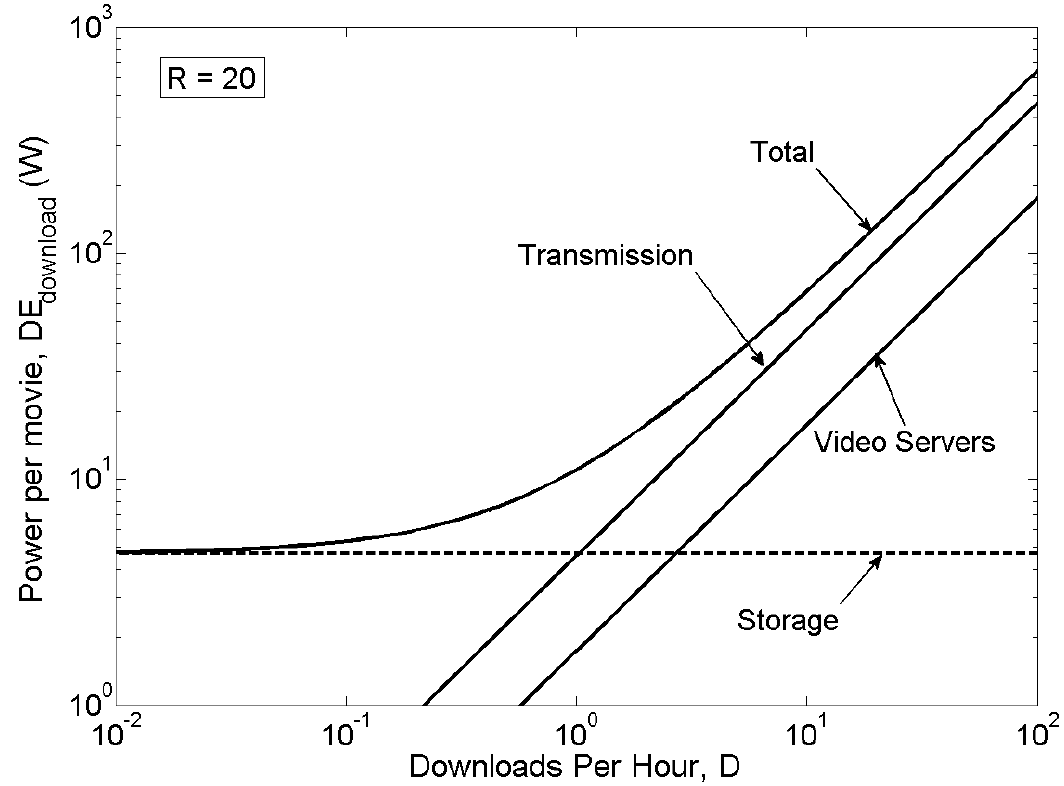
\includegraphics{image/chart7.png}}}
	\caption{The contribution of storage, servers and transmission to the total power consumption of IPTV services with respect to data popularity~\cite{iptv}}.
	\label{fig:popularity}
	\normalsize
\end{figure}

\cite{tradeoff} compared the energy consumption for downloading movies from nano data centers and from centralized data centers with respect to the access frequency,
under the scenario that a centralized data centers keeps two replicas of each data,
and nano data centers keeps 2, or 10, or 100 replicas of each data.
The result indicated that a centralized data center is more efficient than nano data centers for unpopular data.

Thus,
we regard finding the balance between the transmission distance and the number of replicas as one the technical challenges towards the development of nano data centers.
From our view,
a possible solution is to detect the popularity of each individual data dynamically,
and adjusting the number of replicas for each data accordingly.
However,
further study on the negotiation and configuration mechanism is required.







